% !TeX root = ../main.tex
\section{Methodology}
\label{sec:methodology}

\add{The methodology of this work consists of three steps:}
\begin{enumerate}
    \item \add{\emph{Parameter identification.} We identified the parameters
          that can be tuned in an IO500 execution and defined the resulting
          parameter space (Section~\ref{sec:parameter-space}).}
    \item \add{\emph{Reference dataset.} We ran an exhaustive search over this
          space to build a reference dataset in which the best configuration
          is known (Sections~\ref{sec:exhaustive-search} and~\ref{sec:campaign}). Running every
          configuration with the official IO500 settings would have taken
          about 161 days, so the cost of each execution was reduced by
          allowing the benchmark phases to run for less than the 300 seconds
          required by the IO500 rules. The resulting scores are marked as
          \texttt{INVALID}, but all configurations are measured under the
          same conditions.}
    \item \add{\emph{Comparison of the search strategies.} We used this
          dataset to compare random search and Bayesian Optimization with
          different surrogate models, acquisition functions, and budgets
          (Section~\ref{sec:search-strategies}). The strategies were replayed
          offline with the \texttt{-{}-cache-only} option of IOPS, which
          reads the results stored during the exhaustive search instead of
          submitting new jobs.}
\end{enumerate}
\add{Apart from a small number of valid executions used to compare the two
settings, IO500 was therefore executed on the cluster only once, during the
exhaustive search. This saved both core hours and time, and ensured that
every strategy was evaluated on exactly the same measurements.}

\subsection{Parameters}
\label{sec:parameter-space}

The first step of the study was to identify the parameters that \replace{could
affect the performance of}{can be tuned in} an IO500 execution. \del{The
configuration of IO500 contains parameters related to the I/O benchmarks,
but the performance also depends on the execution environment, including
the compute nodes and the parallel file system. We therefore considered
parameters from three main aspects: the IO500 benchmarks, the compute
environment, and the storage system.} \add{We distinguish two classes of
parameters: application-side and system-side. Application-side parameters
are exposed by IO500 itself and control the I/O behaviour of its
benchmarks, together with the resources allocated to the run, namely the
number of compute nodes and the number of processes per node. System-side
parameters, in contrast, tune the behaviour of the parallel file system,
for example the number of storage targets across which the data is
distributed. In Table~\ref{tab:parameter-space}, the IOR, MDTEST, FIND and
Machine categories belong to the application side, and the BeeGFS
category to the system side.}



\add{To identify these parameters, and to retain those that most affect I/O
performance, we relied on the IO500
documentation~\cite{io500running,io500rules} and on previous work. For instance, Ahmad
et al.~\cite{ahmad2025io500} combined recommendations from the literature
with an empirical evaluation to approach an optimal IO500 configuration.
On the file-system side, Boito et al.~\cite{teylo2022beegfs} showed that
the number of storage targets across which a file is striped plays a
central role in the write performance of BeeGFS.} Table~\ref{tab:parameter-space} summarises the parameters identified. \del{ in
these different parts of the system. The role of each group of parameters
is explained in more detail in the following paragraphs.}

\begin{table}[H]
\centering
\caption{Parameters considered in the IO500 tuning study.}
\label{tab:parameter-space}

\rowcolors{2}{gray!10}{white}
\begin{tabular}{lll}
    \hline
    \rowcolor{gray!30}
    \textbf{Category} & \textbf{Parameter} & \textbf{Description} \\
    \hline

    
    IOR & \texttt{transferSize} & Size of each I/O operation \\
    IOR & \texttt{blockSize} & Data handled by each process \\
    IOR & \texttt{filePerProc} & One file per process \\
    
    IOR & \texttt{segmentCount} & Number of file segments \\
    \hline

    MDTEST & \texttt{n} & Number of files per process \\
    MDTEST & \texttt{files-per-dir} & Number of files per directory \\
    \hline

    FIND & \texttt{nproc} & Number of processes \\
    FIND & \texttt{pfind-queue-length} & Size of the work queue \\
    FIND & \texttt{pfind-parallelize...} & Parallel directory access \\
    \hline

    Machine & \texttt{nodes} & Number of compute nodes \\
    Machine & \texttt{processes-per-node} & Number of processes per node \\
    \hline

    BeeGFS & \texttt{ost\_count} & Number of storage targets used \\
    \hline
\end{tabular}


\end{table}



\add{The first category, IOR, groups the parameters of the IOR benchmark,
which IO500 uses for its bandwidth phases. These parameters} \del{the IOR
parameters mainly} control the way data is transferred \replace{during the
bandwidth benchmarks}{during I/O operations, that is, the I/O access
pattern}. The \texttt{transferSize} \add{parameter} determines the amount
of data transferred by each I/O operation. Changing this value can modify
the number of I/O requests sent to the storage system and therefore affect
the measured bandwidth.

The \texttt{blockSize} determines the amount of data \replace{handled by
each process}{written contiguously by each process in each segment}.
Together, \texttt{transferSize} and \texttt{blockSize} define an important
part of the I/O access pattern generated by the benchmark. The
\texttt{filePerProc} parameter determines whether each process works on its
own file or whether several processes access a shared file. This choice
can strongly change the level of contention and the way the parallel file
system handles the benchmark. Finally, \texttt{segmentCount} controls the
number of segments used by the IOR benchmark. Increasing the number of
segments changes the total amount of data processed and the sequence of I/O
operations performed by each process.

\replace{The MDTEST parameters control the metadata benchmark generated by IO500.}{The second category, MDTEST, configures the metadata benchmarks of IO500.}
The parameter \texttt{n} determines the number of files handled by each
process. A larger value therefore generates more file-system metadata
operations. The \texttt{files-per-dir} parameter controls how these files are distributed \replace{between}{across} directories. This can affect performance because
placing many files in the same directory does not generate the same
metadata access pattern as distributing them across several directories.

\replace{The FIND benchmark evaluates}{The third category, FIND, configures the \texttt{find} benchmark, which evaluates} the performance of file discovery operations.
The \texttt{nproc} parameter determines the number of processes involved
in the search and therefore controls the level of parallelism. The \texttt{pfind-queue-length} parameter controls the amount of work that
can be kept in the search queue. The
\texttt{pfind-parallelize-single-dir-access-using-hashing} parameter
\replace{allows accesses to a directory to be distributed between several processes}{uses hashing to distribute the accesses to a single directory across several processes}. These parameters influence how the search work is divided and
executed in parallel.


\replace{The number of compute nodes and the number of processes per node also affect IO500 performance.}{The fourth category, Machine, covers the compute resources allocated to an execution, which also affect IO500 performance.} The \texttt{nodes} parameter determines how many
\texttt{bora} nodes participate in an execution, while
\texttt{processes-per-node} determines how many benchmark processes are
started on each node. Together, these two parameters determine the total number of processes
accessing the storage system. Increasing this number can provide more I/O
parallelism, but it can also increase contention when many processes \replace{access the storage system simultaneously}{issue requests at the same time}.


\add{The fifth and last category, BeeGFS, is the only system-side one.} The experiments use BeeGFS as the parallel file system. The
\texttt{ost\_count} parameter controls the number of storage targets \replace{used to distribute file data}{across which file data is striped}. Using a larger number of targets can \replace{distribute I/O operations across}{spread I/O operations over} more storage resources and potentially increase the available bandwidth\add{~\cite{teylo2022beegfs}}.
However, the best value depends on the benchmark and on the number of
processes accessing the storage system. The effect of this parameter must
therefore be considered together with the IOR and \replace{compute}{Machine} parameters.


These parameters do not act independently. For example, increasing the
number of processes can change the benefit obtained from using more
storage targets, while the effect of a given \texttt{transferSize} can
depend on the level of parallelism used during the execution. A configuration is therefore defined by \replace{a combination of values from the different parameter categories}{one value for each parameter of Table~\ref{tab:parameter-space}}. The set of all possible combinations
forms the parameter space of the study. Exploring this space makes it
possible to study the interactions between parameters and to identify
configurations that provide high IO500 scores. \del{However, the number of possible combinations quickly becomes large. This
makes a complete evaluation expensive when each configuration requires an
IO500 execution. The following sections describe how this parameter space
was explored and how a reduced-cost exhaustive campaign was used as a
reference for the evaluation of the search strategies.}


\subsection{Building the reference dataset}
\label{sec:exhaustive-search}

\note{Paragraph headings removed so the subsection reads as one continuous
account. The description of the IOPS campaign now forms
Section~\ref{sec:campaign}.}

\del{The first approach used in this study was exhaustive search. The idea was
to test every possible configuration in the parameter space in order to
identify the best IO500 configuration.}

\del{The goal of this work is not to use exhaustive search as a practical
tuning method. Testing all configurations is too expensive for this
purpose. Instead, exhaustive search is used to create a reference dataset.
This reference contains the results of all tested configurations and can
later be used to compare Random Search and the different Bayesian
Optimization methods.}

\add{Once the parameters were identified, the reference dataset had to be
built by evaluating every configuration of the parameter space.}
The most direct way to build this reference would be to run every
configuration using the official IO500 settings. However, this would take
too much time.
Before starting the experiments, IOPS was used to estimate the execution
time required for the complete exhaustive search. With valid IO500
executions, the estimated duration was approximately 161 days.

\note{Figure with the IOPS time estimate removed; the 161-day estimate is
given in the text.}

This duration was close to the complete length of the internship, which
lasted five months. In addition, the experiments were executed on the
PlaFRIM \texttt{bora} nodes. These nodes are shared with other users.
Running the complete exhaustive search with valid IO500 executions would
therefore require using and reserving compute resources for a very long
period. This was not practical on a shared research platform.
For this reason, a faster way to evaluate the configurations was needed.
\del{The idea was to reduce the cost of each IO500 execution.}

Two main changes were made. First, the stonewall time was reduced from
300 seconds to 10 seconds. Second, \replace{the size-related parameters used in the benchmark were divided by 10}{the
amount of work of each phase was reduced: the total volume of data written
by \texttt{ior-easy} was set to 30~GiB, the number of segments of
\texttt{ior-hard} to 1\,000, and the number of files per process of the
MDTEST benchmarks to 100 (Table~\ref{tab:exhaustive-values})}. These changes reduced the amount of
work performed during each execution and made the tests much faster.
With these reduced settings, some IO500 phases do not satisfy the
official execution requirements. The final IO500 result is therefore
marked as \texttt{INVALID}. These results cannot be used as official
IO500 submissions. \add{Figure~\ref{fig:io500-invalid-run} shows the output of
one such execution.}

\begin{figure}[H]
    \centering
    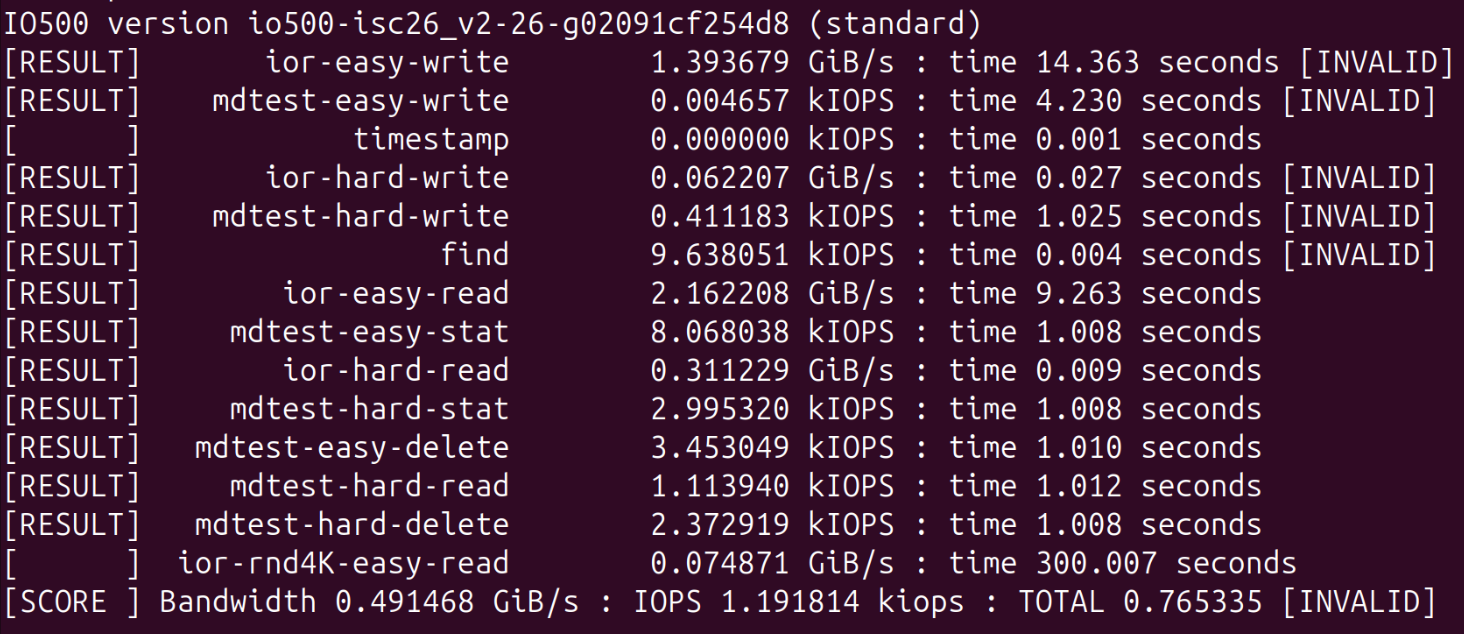
\includegraphics[width=0.95\textwidth]{figures/io500_invalid_run.png}
    \caption{Output of a reduced-cost IO500 execution. The write phases and
    the \texttt{find} phase end after a few seconds, far below the 300
    seconds required by the IO500 rules, and are flagged as
    \texttt{INVALID}, which also invalidates the final score.}
    \label{fig:io500-invalid-run}
\end{figure}

However, the purpose of these short tests is not to produce an official
IO500 score. Their purpose is to provide a cheaper way to compare
configurations under the same experimental conditions.

The main question was therefore whether these short executions could
still give useful information about the quality of a configuration. In
particular, we wanted to know whether configurations that perform well
with the reduced settings also tend to perform well with valid IO500
settings. \add{This question is examined in Section~\ref{sec:valid-invalid}.}
\replace{For this reason, the}{The} reduced settings were used for the exhaustive
search. All configurations were evaluated under the same conditions,
which makes their results comparable within this study.

\note{The comparison between valid and invalid executions, with its
figure, was moved to Section~\ref{sec:valid-invalid}: it is a result
rather than part of the method.}

\add{Beyond the cost of each execution, the measurements also had to account for performance variability.} I/O performance can vary between executions, even when the same
configuration is used. Temporary activity on the compute or storage
system can affect the measured performance.
For this reason, each configuration was executed three times. These
repetitions reduce the effect of temporary variations and provide more
information about the stability of each configuration.
The exhaustive search contained 4,830 possible configurations. With
three repetitions for each configuration, the complete experiment
therefore represented 14\,490 IO500 executions.
\del{All repetitions used the same reduced-cost settings, including the
10-second stonewall time and the reduced size-related parameters.}

\subsection{Running the campaign with IOPS}
\label{sec:campaign}
\label{sec:ground-truth}

\note{New subsection: the IOPS campaign was previously part of
Section~\ref{sec:exhaustive-search}. Its closing part, on the reference
dataset, comes from the former ground-truth subsection.}

\add{This subsection describes how the exhaustive search was run with IOPS:
the definition of the parameter space, the generation and submission of
the jobs, and the collection of the results that form the reference
dataset.}

The experiments were defined using a YAML configuration file interpreted
by IOPS. This file contains the benchmark settings, the parameter values,
the execution method, the SLURM configuration, and the way the results
are collected.
\add{The \texttt{vars} and \texttt{constraints} sections of this file define
the parameter space of the study. They are reproduced below.}

\note{The complete \texttt{vars} and \texttt{constraints} sections, as
generated by the study scripts for the whole measured grid, replace the
partial excerpts shown before (a single constraint and the
\texttt{repetitions} line) and the two formulas for \texttt{ntasks} and the
block size.}

\begin{minted}[
    fontsize=\small,
    frame=lines,
    breaklines=true
]{yaml}
vars:
  nodes:
    type: int
    sweep: {mode: list, values: [1, 2, 4, 6, 8, 10, 16]}
  processes_per_node:
    type: int
    sweep: {mode: list, values: [8, 16, 24, 32, 36]}
  transfer_size_mb:
    type: int
    sweep: {mode: list, values: [1, 2, 4, 8, 16, 32, 64]}
  ost_count:
    type: int
    sweep: {mode: list, values: [1, 2, 3, 4, 5, 6, 7, 8]}
  file_per_proc:
    type: bool
    sweep: {mode: list, values: [true, false]}
  unique_dir:
    type: bool
    sweep: {mode: list, values: [true, false]}
  total_size_gb:
    type: int
    expr: "30"
  segment_count:
    type: int
    expr: "1000"
  files_per_proc:
    type: int
    expr: "100"
  pfind_queue_size:
    type: int
    expr: "100"
  ntasks:
    type: int
    expr: "{{ nodes * processes_per_node }}"
  block_size_mb:
    type: int
    expr: "{{ (total_size_gb*1024) // ntasks }}"
  ost_folder:
    type: str
    expr: "/beegfs/lgouveia/ior_{{ost_count}}/datafiles"

constraints:
  - name: align
    rule: "block_size_mb % transfer_size_mb == 0"
    violation_policy: skip
  - name: ge
    rule: "block_size_mb >= transfer_size_mb"
    violation_policy: skip
\end{minted}

\add{Each entry of the \texttt{vars} section defines one variable. The
variables with a \texttt{sweep} are the explored parameters: IOPS takes every
value in their list, and the parameter space is the Cartesian product of
these lists. The six swept variables are the parameters selected in
Section~\ref{sec:parameter-space}: the number of compute nodes, the number of
processes per node, the transfer size, the number of storage targets, and
the two Boolean options \texttt{file\_per\_proc} and \texttt{unique\_dir},
which set the \texttt{filePerProc} and \texttt{uniqueDir} options of
\texttt{ior-easy}.}

\add{The variables defined by a constant \texttt{expr} are not explored. They
fix the size of the workload and therefore define the reduced-cost setting
described above: \texttt{total\_size\_gb} sets the volume of data written by
\texttt{ior-easy} to 30~GiB, \texttt{segment\_count} sets the
\texttt{segmentCount} of \texttt{ior-hard} to 1\,000, \texttt{files\_per\_proc}
sets the number of files per process \texttt{n} of both MDTEST phases to
100, and \texttt{pfind\_queue\_size} sets the work queue of \texttt{find} to
100.}

\add{The remaining variables are derived from the swept values and are
evaluated by IOPS for each configuration, using the Jinja syntax
\texttt{\{\{~\ldots~\}\}}. The variable \texttt{ntasks} is the total number
of MPI processes. The variable \texttt{block\_size\_mb} divides the 30~GiB
evenly between these processes, so the total volume written does not depend
on the number of processes. Finally, \texttt{ost\_folder} selects the
directory in which IO500 writes its data. The BeeGFS directories
\texttt{ior\_1} to \texttt{ior\_8} were prepared with a stripe count of one to
eight storage targets, so selecting the directory is how the value of
\texttt{ost\_count} is applied.}

\add{Not every combination of these values is a valid IOR configuration. The
two constraints discard the combinations in which the block size is not a
multiple of the transfer size (\texttt{align}) or is smaller than it
(\texttt{ge}). With \texttt{violation\_policy: skip}, IOPS drops these
combinations before any job is submitted, so no cluster time is spent on
them.}

\begin{cut}
The parameters that have to be explored are defined in the
\texttt{vars} section. For example, the number of nodes, the number of
processes per node, the transfer size, the number of storage targets,
\texttt{file\_per\_proc}, and \texttt{unique\_dir} can each take several
values.
\end{cut}

\add{Table~\ref{tab:exhaustive-values} summarises these values.}

\begin{table}[H]
\centering
\caption{Values used in the exhaustive search. The explored parameters form
the parameter space, the derived parameters are computed by IOPS for each
configuration, and the fixed parameters define the reduced-cost setting.}
\label{tab:exhaustive-values}
\rowcolors{2}{gray!10}{white}
\begin{tabular}{lll}
    \hline
    \rowcolor{gray!30}
    \textbf{Parameter} & \textbf{Option} & \textbf{Values} \\
    \hline
    \multicolumn{3}{l}{\cellcolor{white}\textit{Explored}} \\
    Compute nodes & \texttt{nodes} & 1, 2, 4, 6, 8, 10, 16 \\
    Processes per node & \texttt{processes\_per\_node} & 8, 16, 24, 32, 36 \\
    Transfer size (MiB) & \texttt{transferSize} & 1, 2, 4, 8, 16, 32, 64 \\
    Storage targets & \texttt{ost\_count} & 1 to 8 \\
    One file per process & \texttt{filePerProc} & true, false \\
    Unique directory per process & \texttt{uniqueDir} & true, false \\
    \hline
    \multicolumn{3}{l}{\cellcolor{white}\textit{Derived}} \\
    MPI tasks & \texttt{ntasks} & nodes $\times$ processes per node \\
    Block size (MiB) & \texttt{blockSize} & $30 \times 1024\,/\,$\texttt{ntasks} \\
    \hline
    \multicolumn{3}{l}{\cellcolor{white}\textit{Fixed (reduced-cost setting)}} \\
    Stonewall time & \texttt{stonewall-time} & 10\,s (300\,s for a valid run) \\
    Data volume of \texttt{ior-easy} & \texttt{total\_size\_gb} & 30\,GiB \\
    Segments of \texttt{ior-hard} & \texttt{segmentCount} & 1\,000 \\
    Files per process (MDTEST) & \texttt{n} & 100 \\
    Work queue of \texttt{find} & \texttt{pfind-queue-length} & 100 \\
    Repetitions & \texttt{repetitions} & 3 \\
    \hline
\end{tabular}
\end{table}

\del{Some parameters are not explored directly but are computed from other
parameters. For example, the total number of MPI tasks is calculated as:}
\del{The block size is also computed from the total data size and the number
of tasks:}
\del{IOPS can also apply constraints before running a configuration. In this
study, the block size had to be a multiple of the transfer size. Invalid
combinations were skipped automatically:}
\del{This is important because not every mathematical combination of the
parameter values represents a valid IO500 configuration.}

The YAML file is also used to generate the IO500 configuration file for
each execution. IOPS replaces the parameter values in the template before
submitting the job. For example, the transfer size, block size,
file-per-process option, and storage directory are generated from the
values selected for the current configuration. \add{The template used in this study is the
following:}

\begin{minted}[
    fontsize=\small,
    frame=lines,
    breaklines=true
]{yaml}
scripts:
  - name: "IO500"
    inputs:
      - name: config_ini
        path: "{{ execution_dir }}/config.ini"
        template: |
          [global]
          datadir = {{ ost_folder }}
          timestamp-datadir = TRUE
          resultdir = {{ execution_dir }}/results
          timestamp-resultdir = FALSE
          api = POSIX
          io-buffers-on-gpu = FALSE
          verbosity = 1
          scc = FALSE
          dataPacketType = timestamp

          [debug]
          stonewall-time = 10

          [ior-easy]
          transferSize = {{transfer_size_mb}}m
          blockSize = {{ block_size_mb }}m
          filePerProc = {% if  file_per_proc == true %}TRUE{% else %}FALSE{% endif %}

          uniqueDir = {%if unique_dir == true %}TRUE{% else %}FALSE{% endif %}

          run = TRUE

          [mdtest-easy]
          API = POSIX
          n = {{files_per_proc}}
          run = TRUE

          [ior-hard]
          API = POSIX
          segmentCount = {{ segment_count }}
          run = TRUE

          [mdtest-hard]
          API = POSIX
          n = {{files_per_proc}}
          run = TRUE

          [find]
          run = TRUE
          pfind-queue-length = {{pfind_queue_size}}
          pfind-steal-next = FALSE
          pfind-parallelize-single-dir-access-using-hashing = FALSE
\end{minted}

\add{The template follows the IO500 configuration format, with one section
per benchmark phase. Each placeholder between double braces is replaced by
the value of the corresponding variable of the \texttt{vars} section: the
transfer size and block size of \texttt{ior-easy}, the size parameters of
the reduced-cost setting, and the directory \texttt{ost\_folder}, which
determines the number of storage targets used. The Jinja conditions
\texttt{\{\%~if~\ldots~\%\}} translate the two Boolean variables into the
\texttt{TRUE} and \texttt{FALSE} values expected by IO500. The
\texttt{[debug]} section sets the stonewall time to 10 seconds, which,
together with the reduced size parameters, makes each execution a
reduced-cost one. All five benchmarks are enabled with \texttt{run = TRUE},
so every execution produces a complete IO500 score.}

The execution itself is submitted to SLURM. The job script defines the
number of nodes, the total number of MPI tasks, and the number of
processes per node. The jobs are executed on the PlaFRIM
\texttt{bora} nodes using an exclusive allocation.
\replace{Each configuration is executed three times, as defined by:}{Each
configuration is executed three times, as set by the \texttt{repetitions}
option of the benchmark section.}

The search strategy is also selected directly in the YAML file. This
means that the same benchmark definition can be used with Exhaustive
Search, Random Search, or Bayesian Optimization by changing the search
method while keeping the rest of the experimental setup unchanged.

\add{The last part of the process was the collection of the results.} After each execution, IOPS parses the IO500 output and extracts the main
performance metrics. In this study, the parser collects the overall
IO500 score, the bandwidth result, and the metadata result:

\begin{minted}[
    fontsize=\small,
    frame=lines,
    breaklines=true
]{yaml}
parser:
  file: "{{ execution_dir }}/results/result.txt"
  metrics:
    - name: SCORE
    - name: BW
    - name: MD

  parser_script: |
    import re

    def parse(file_path: str):
      result = {
        "SCORE": None,
        "BW": None,
        "MD": None,
      }
      with open(file_path, "r") as f:
        for x in f:
          x = x.strip()

          m = re.search(r"SCORE\s*=\s*(\S+)", x)
          if m:
            result["SCORE"] = float(m.group(1))
            continue

          m = re.search(r"BW\s*=\s*(\S+)", x)

          if m:
            result["BW"] = float(m.group(1))
            continue

          m = re.search(r"MD\s*=\s*(\S+)", x)
          if m:
            result["MD"] = float(m.group(1))
            continue

      return result
\end{minted}

\note{The excerpt was extended to the complete parser definition of the
campaign configuration.}

\add{The parser tells IOPS where to find the output of IO500 and how to read
it. The \texttt{file} entry points to the \texttt{result.txt} file written
by IO500 in the results directory of each execution, and the
\texttt{metrics} list declares the three values to extract. The
\texttt{parser\_script} is a short Python function that IOPS calls on this
file. It reads the file line by line and uses regular expressions to find
the lines containing \texttt{SCORE =}, \texttt{BW =} and \texttt{MD =},
which IO500 writes at the end of an execution, and returns their numerical
values. A value that is not found is returned as \texttt{None}.}

IOPS also stores information about the configuration and the execution.
At the end of the experiment, these values are written to a CSV file,
with one row for each execution.
The result file contains several groups of columns. The
\texttt{vars.*} columns describe the configuration used for the
execution. They include, for example,
\texttt{vars.nodes},
\texttt{vars.processes\_per\_node},
\texttt{vars.transfer\_size\_mb},
\texttt{vars.ost\_count},
\texttt{vars.file\_per\_proc}, and
\texttt{vars.unique\_dir}.
The \texttt{execution.*} columns identify the execution and its
repetition. The \texttt{metadata.*} columns contain information about
the SLURM job and the machine on which it was executed. Finally, the
\texttt{metrics.*} columns contain the IO500 results, in particular
\texttt{metrics.SCORE}, \texttt{metrics.BW}, and
\texttt{metrics.MD}.

This CSV file therefore gives, for every execution, both the parameter
values that were used and the performance obtained with these values.
It is the main source of data used to build the reference dataset for the
rest of the study.
\del{The exhaustive search produced a large number of IO500 results for the
parameter space used in this study. These results were then used to build
a reference dataset for comparing the different search methods.}

\begin{cut}
For each execution, IOPS stores the parameter values and the corresponding
IO500 results. The main information used in this study includes the
configuration parameters, the repetition number, and the three main
metrics: \texttt{SCORE}, \texttt{BW}, and \texttt{MD}.
\end{cut}

\del{Each configuration was executed three times. This provides several
measurements for the same configuration and helps reduce the effect of
temporary performance variations. It also gives a more reliable view of
the performance of each configuration.}



\subsection{Evaluation of the search strategies}
\label{sec:search-strategies}

\note{Paragraph headings removed, as in Section~\ref{sec:exhaustive-search}.
The offline evaluation and the comparison with the reference come from the
former ground-truth subsection; the evaluation protocol and the list of BO
configurations were added from the study scripts.}

\add{The third step of the methodology uses the reference dataset to
compare the search strategies. The strategies are not executed on the
cluster: they are replayed on the results stored during the exhaustive
search, as described below.}
The results were also stored in the IOPS cache file
\texttt{io500.db}. The cache links each configuration to the result
already measured for it.
This is useful when comparing Random Search and Bayesian Optimization.
When a search method selects a configuration, there is no need to run
IO500 again. IOPS can directly read the result from the cache.
The \texttt{-{}-cache-only} option was used for this purpose. With this
option, IOPS only uses results already stored in the cache and does not
submit new jobs to the cluster.
This makes it possible to repeat the search experiments many times
without using additional \texttt{bora} resources. It also ensures that
all search methods are compared using the same IO500 measurements.
\del{The reference dataset and the cache are therefore used for the offline
comparison of the search methods described in the next section.}

\add{Each strategy was evaluated with a fixed budget, defined as the maximum
number of configurations it is allowed to evaluate. For each evaluated
configuration, IOPS reads its three cached repetitions. The quality of a
run is the best SCORE observed among the executions it read, and its cost
is the sum of their measured durations, that is, the wall-clock time the
run would have spent on the cluster. Random Search and Bayesian
Optimization are stochastic, so every setting was run with ten different
random seeds, and the results are reported as the mean and standard
deviation over these ten runs.}

\replace{This reference is}{The reference dataset is} then used to evaluate the search methods. For example,
if Bayesian Optimization is allowed to test only 40 configurations, the
best configuration it finds can be compared with the best configuration
in the complete reference dataset. This shows how close the method gets
to the best known result with only a small number of evaluations.
\add{In the results, this distance is expressed as a percentage of the best SCORE of the dataset.}

    \subsubsection{Random Search}
\label{sec:random-search}

Random Search was used as a simple search method in this study. Instead
of testing every possible configuration, it selects a subset of the
parameter space at random.
In IOPS, Random Search is enabled directly in the YAML configuration by
setting:

\begin{minted}[
    fontsize=\small,
    frame=lines,
    breaklines=true
]{yaml}
search_method: "random"
\end{minted}

\replace{The amount of the parameter space to explore can also be defined in the
Random Search configuration.}{The number of configurations to evaluate is set
in the Random Search configuration.} For example:

\begin{minted}[
    fontsize=\small,
    frame=lines,
    breaklines=true
]{yaml}
random_config:
  n_samples: 40
\end{minted}

\note{Example changed from \texttt{percentage: 0.05} to \texttt{n\_samples},
the option used in the study.}

\begin{cut}
In this example, Random Search selects 5\% of the available
configurations. Other percentages can be used depending on the number of
configurations that should be evaluated.
\end{cut}

\add{In this example, Random Search evaluates 40 configurations. In this
study, it was run with budgets of 10, 15, 20, 30, 40, 60, 80, and 120
configurations, which covers the same range as the budgets used for Bayesian Optimization.}
The selected configurations come from the same parameter space defined
for the study. The same constraints are applied, so configurations that
do not satisfy the experimental rules are not considered.
Random Search does not use the results of previous executions to choose
new configurations. The configurations are selected randomly from the
available search space.
This makes Random Search simple to configure and allows only a part of
the complete parameter space to be evaluated. \add{It is therefore used as the baseline against which Bayesian Optimization is compared.}


\subsubsection{Bayesian Optimization}
\label{sec:bayesian-search}

Bayesian Optimization was the main guided search method studied during
the internship. Unlike Random Search, it uses the results of previous
evaluations to decide which configuration should be tested next.
\replace{In IOPS, Bayesian Optimization is enabled by setting:}{In IOPS,
Bayesian Optimization is enabled and configured in the \texttt{benchmark}
section of the YAML file. The configuration of the best setup found in this
study is shown below; the paths and monitoring options are omitted.}

\note{The separate YAML excerpts of this subsection were replaced by the
complete configuration of one setup, taken from the study scripts, and by
Table~\ref{tab:bo-values}.}

\begin{minted}[
    fontsize=\small,
    frame=lines,
    breaklines=true
]{yaml}
benchmark:
  repetitions: 3
  search_method: "bayesian"
  random_seed: 0
  bayesian_config:
    objective_metric: "SCORE"
    objective: "maximize"
    n_initial_points: 5
    n_iterations: 40
    acquisition_func: "LCB"
    base_estimator: "GP"
    xi: 0.01
    kappa: 1.96
    fallback_to_exhaustive: false
\end{minted}

\begin{cut}
The objective of the search is also defined in the configuration. In this
study, the IO500 \texttt{SCORE} is the value to maximise:
\end{cut}

\add{The \texttt{objective\_metric} and \texttt{objective} options define
the value to optimise: in this study, the IO500 SCORE is maximised. The
\texttt{random\_seed} option initialises the random choices made during the
search, so a run can be reproduced exactly; each setup was run with the
seeds 0 to 9. Finally, \texttt{fallback\_to\_exhaustive} is disabled. When
this option is enabled, IOPS replaces the search by an exhaustive one if the
budget is at least as large as the parameter space; disabling it guarantees
that the optimiser is always used. The other options of
\texttt{bayesian\_config} define the variant of Bayesian Optimization and
are described below.}

Bayesian Optimization starts by evaluating a small number of initial
configurations. These first results are used to build a model of the
relation between the parameter values and the IO500 score. The model is
then used to select the next configuration. After this configuration is
evaluated, the new result is added to the previous observations and the
model is updated. This process continues until the evaluation budget is
reached\add{, as described in Section~\ref{sec:background-bo}}.
Bayesian Optimization is not a single fixed method. Several choices can
be made for the model and for the strategy used to select the next
configuration. In IOPS, these choices are controlled by the
\texttt{bayesian\_config} section.

\add{The first choice concerns the surrogate model.} The surrogate model estimates the IO500 score of configurations that have
not yet been evaluated. Three surrogate models were considered in this
study:

\begin{itemize}
    \item \texttt{GP}: Gaussian Process;
    \item \texttt{RF}: Random Forest;
    \item \texttt{ET}: Extra Trees.
\end{itemize}
All three models learn from the configurations already evaluated, but
they represent the relation between parameters and performance in
different ways. The choice of surrogate model can therefore change the
configurations proposed during the search.
The model is selected with the \texttt{base\_estimator} option. \del{For example:} \del{selects a Random Forest as the surrogate model.}

Once the surrogate model has been built, an acquisition function is used
to choose the next configuration to evaluate. Three acquisition
functions were considered:

\begin{itemize}
    \item \texttt{EI}: Expected Improvement;
    \item \texttt{PI}: Probability of Improvement;
    \item \texttt{LCB}: Lower Confidence Bound.
\end{itemize}
EI considers the expected improvement over the best result found so far.
PI considers the probability that a configuration will improve the
current best result. LCB uses the prediction of the model together with
its uncertainty to decide where to search next.

\del{These functions provide different ways to balance two important
behaviours. The first is exploitation, which means testing configurations
that are expected to perform well. The second is exploration, which means
testing less-known parts of the parameter space.} \add{As explained in
Section~\ref{sec:background-bo}, they differ in how they balance
exploitation and exploration.}
\replace{The acquisition function is selected with, for example:}{The
acquisition function is selected with the \texttt{acquisition\_func}
option.}

The balance between exploration and exploitation can also be controlled
by additional parameters.
For EI and PI, the parameter \texttt{xi} controls the amount of
exploration. Different values can therefore make the search more focused
on the current best region or encourage it to explore other parts of the
parameter space.
For LCB, this role is controlled by \texttt{kappa}. A larger value gives
more importance to uncertainty and therefore encourages more exploration.
\del{For example, a BO configuration can use:}
Only the parameter related to the selected acquisition function has an
effect on the search.

\add{Finally, two options control the size of the search.} The parameter \texttt{n\_initial\_points} defines how many configurations
are evaluated before the surrogate model starts guiding the search. These
initial configurations provide the first observations needed to build the
model.
The parameter \texttt{n\_iterations} controls the number of evaluations
performed by the optimisation. \replace{It therefore represents an important part of the search budget.}{It therefore defines the evaluation budget, including the initial points.} A larger budget gives Bayesian Optimization more
opportunities to learn about the parameter space, but it also requires
more evaluations. \del{For example:} \del{starts the optimisation with five initial points
and uses an evaluation budget defined by ten iterations.}

\del{The following configuration is one example of a Bayesian Optimization
setup used with IOPS:}

\begin{cut}
This example corresponds to a Random Forest surrogate combined with the
Expected Improvement acquisition function. It uses five initial points
and \texttt{xi = 0.01}. This is only one possible BO configuration.
\end{cut}

In this study, several combinations of surrogate models, acquisition
functions, exploration parameters, initial points, and evaluation budgets
were tested. This is important because changing one of these options can
change the behaviour of Bayesian Optimization. The goal was therefore not
only to test whether Bayesian Optimization works for IO500, but also to
determine which BO configuration is the most effective for this problem.

\add{The configurations were organised in two groups. The main grid combines
the three surrogate models with five acquisition settings, namely EI with
\texttt{xi}~=~0.01 and 0.1, PI with \texttt{xi}~=~0.01, and LCB with
\texttt{kappa}~=~1.96 and 5.0, and with nine budgets of 10, 15, 20, 30, 40, 60, 80, 100, and 120
evaluations, always starting from five initial points. This gives
$3 \times 5 \times 9 = 135$ setups. A sensitivity analysis then varies one
option at a time around a default setup (Random Forest, EI,
\texttt{xi}~=~0.01, five initial points) at budgets of 20 and 40
evaluations: the surrogate model, the acquisition function, \texttt{xi} in
$\{0.001, 0.01, 0.1\}$, \texttt{kappa} in $\{0.5, 1.96, 5.0\}$, and the
number of initial points in $\{3, 5, 10\}$. Most of these settings are
already part of the main grid; only \texttt{xi}~=~0.001,
\texttt{kappa}~=~0.5, and three or ten initial points are new, which adds 8
setups. In total, 143 BO setups were evaluated, each with the ten seeds, for 1\,430 searches. Table~\ref{tab:bo-values} summarises the values taken by each
option.}

\begin{table}[H]
\centering
\caption{Options of Bayesian Optimization varied in this study. Only the
exploration parameter of the selected acquisition function is active:
\texttt{xi} for EI and PI, \texttt{kappa} for LCB.}
\label{tab:bo-values}
\rowcolors{2}{gray!10}{white}
\begin{tabular}{lll}
    \hline
    \rowcolor{gray!30}
    \textbf{Option} & \textbf{Role} & \textbf{Values} \\
    \hline
    \texttt{base\_estimator} & Surrogate model & GP, RF, ET \\
    \texttt{acquisition\_func} & Acquisition function & EI, PI, LCB \\
    \texttt{xi} & Exploration (EI, PI) & 0.001, 0.01, 0.1 \\
    \texttt{kappa} & Exploration (LCB) & 0.5, 1.96, 5.0 \\
    \texttt{n\_initial\_points} & Initial configurations & 3, 5, 10 \\
    \texttt{n\_iterations} & Evaluation budget & 10 to 120 (nine values) \\
    \texttt{random\_seed} & Seed of each run & 0 to 9 \\
    \hline
\end{tabular}
\end{table}

IOPS implements the Bayesian search as a sequential process. At each
iteration, the optimiser suggests a new point based on the results
already available. IOPS then maps this suggestion to a valid
configuration from the parameter space. The result of this configuration
is returned to the optimiser and used to update the model.
The process can therefore be summarised as:

\[
\text{suggest}
\rightarrow
\text{select a valid configuration}
\rightarrow
\text{evaluate}
\rightarrow
\text{update the model}.
\]
Because each new suggestion depends on the previous results, Bayesian
Optimization is sequential: the result of one evaluation is used before
selecting the next configuration.